% DiffLaR Teaser Figure - Comparison of Reasoning Paradigms
\documentclass[tikz,border=10pt]{standalone}
\usepackage{tikz}
\usetikzlibrary{shapes,arrows,positioning,fit,backgrounds,calc,decorations.pathreplacing}

\definecolor{tokenblue}{RGB}{66,133,244}
\definecolor{latentgreen}{RGB}{52,168,83}
\definecolor{diffpurple}{RGB}{156,39,176}
\definecolor{queryorange}{RGB}{251,188,5}

\begin{document}
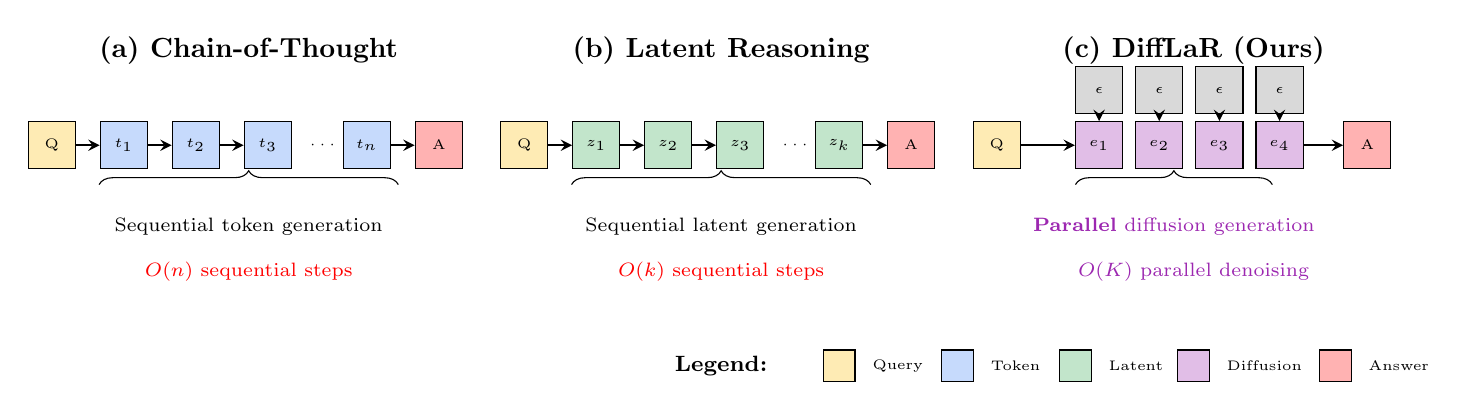
\begin{tikzpicture}[
    node distance=0.3cm,
    token/.style={rectangle, draw, fill=tokenblue!30, minimum width=0.6cm, minimum height=0.6cm, font=\tiny},
    latent/.style={rectangle, draw, fill=latentgreen!30, minimum width=0.6cm, minimum height=0.6cm, font=\tiny},
    difflatent/.style={rectangle, draw, fill=diffpurple!30, minimum width=0.6cm, minimum height=0.6cm, font=\tiny},
    query/.style={rectangle, draw, fill=queryorange!30, minimum width=0.6cm, minimum height=0.6cm, font=\tiny},
    answer/.style={rectangle, draw, fill=red!30, minimum width=0.6cm, minimum height=0.6cm, font=\tiny},
    arrow/.style={->, >=stealth, thick},
    brace/.style={decorate, decoration={brace, amplitude=5pt}}
]

% (a) Chain-of-Thought
\node[font=\bfseries] at (0, 2) {(a) Chain-of-Thought};

\node[query] (q1) at (-2.5, 0.8) {Q};
\node[token, right=of q1] (t1) {$t_1$};
\node[token, right=of t1] (t2) {$t_2$};
\node[token, right=of t2] (t3) {$t_3$};
\node[right=0.1cm of t3, font=\tiny] {$\cdots$};
\node[token] (tn) at (1.5, 0.8) {$t_n$};
\node[answer, right=of tn] (a1) {A};

\draw[arrow] (q1) -- (t1);
\draw[arrow] (t1) -- (t2);
\draw[arrow] (t2) -- (t3);
\draw[arrow] (tn) -- (a1);

\draw[brace] (-1.9, 0.3) -- (1.9, 0.3) node[midway, below=0.3cm, font=\scriptsize] {Sequential token generation};

% (b) Latent Reasoning (Autoregressive)
\node[font=\bfseries] at (6, 2) {(b) Latent Reasoning};

\node[query] (q2) at (3.5, 0.8) {Q};
\node[latent, right=of q2] (l1) {$z_1$};
\node[latent, right=of l1] (l2) {$z_2$};
\node[latent, right=of l2] (l3) {$z_3$};
\node[right=0.1cm of l3, font=\tiny] {$\cdots$};
\node[latent] (lk) at (7.5, 0.8) {$z_k$};
\node[answer, right=of lk] (a2) {A};

\draw[arrow] (q2) -- (l1);
\draw[arrow] (l1) -- (l2);
\draw[arrow] (l2) -- (l3);
\draw[arrow] (lk) -- (a2);

\draw[brace] (4.1, 0.3) -- (7.9, 0.3) node[midway, below=0.3cm, font=\scriptsize] {Sequential latent generation};

% (c) DiffLaR (Parallel)
\node[font=\bfseries] at (12, 2) {(c) DiffLaR (Ours)};

\node[query] (q3) at (9.5, 0.8) {Q};

% Noise to latent
\node[difflatent, fill=gray!30] (n1) at (10.8, 1.5) {$\epsilon$};
\node[difflatent, fill=gray!30, right=0.15cm of n1] (n2) {$\epsilon$};
\node[difflatent, fill=gray!30, right=0.15cm of n2] (n3) {$\epsilon$};
\node[difflatent, fill=gray!30, right=0.15cm of n3] (n4) {$\epsilon$};

\node[difflatent] (d1) at (10.8, 0.8) {$e_1$};
\node[difflatent, right=0.15cm of d1] (d2) {$e_2$};
\node[difflatent, right=0.15cm of d2] (d3) {$e_3$};
\node[difflatent, right=0.15cm of d3] (d4) {$e_4$};

\node[answer, right=0.5cm of d4] (a3) {A};

\draw[arrow] (q3) -- (d1);
\draw[arrow, dashed] (n1) -- (d1);
\draw[arrow, dashed] (n2) -- (d2);
\draw[arrow, dashed] (n3) -- (d3);
\draw[arrow, dashed] (n4) -- (d4);
\draw[arrow] (d4) -- (a3);

% Parallel indicator
\draw[brace] (10.5, 0.3) -- (13.0, 0.3) node[midway, below=0.3cm, font=\scriptsize, text=diffpurple] {\textbf{Parallel} diffusion generation};

% Time complexity labels
\node[font=\scriptsize, text=red] at (0, -0.8) {$O(n)$ sequential steps};
\node[font=\scriptsize, text=red] at (6, -0.8) {$O(k)$ sequential steps};
\node[font=\scriptsize, text=diffpurple] at (12, -0.8) {$O(K)$ parallel denoising};

% Legend
\begin{scope}[shift={(6, -2)}]
    \node[font=\footnotesize\bfseries] at (0, 0) {Legend:};
    \node[query, minimum width=0.4cm, minimum height=0.4cm] at (1.5, 0) {};
    \node[font=\tiny, right] at (1.8, 0) {Query};
    \node[token, minimum width=0.4cm, minimum height=0.4cm] at (3, 0) {};
    \node[font=\tiny, right] at (3.3, 0) {Token};
    \node[latent, minimum width=0.4cm, minimum height=0.4cm] at (4.5, 0) {};
    \node[font=\tiny, right] at (4.8, 0) {Latent};
    \node[difflatent, minimum width=0.4cm, minimum height=0.4cm] at (6, 0) {};
    \node[font=\tiny, right] at (6.3, 0) {Diffusion};
    \node[answer, minimum width=0.4cm, minimum height=0.4cm] at (7.8, 0) {};
    \node[font=\tiny, right] at (8.1, 0) {Answer};
\end{scope}

\end{tikzpicture}
\end{document}
